\ifx\wholebook\relax \else

\documentclass[b5paper]{ctexart}

\usepackage[cn]{../../prelude}

\setcounter{page}{1}

\begin{document}

\title{前言}

\author{刘新宇
\thanks{{\bfseries 刘新宇} \newline
  Email: liuxinyu95@gmail.com \newline}
  }

\maketitle
\fi

\markboth{前言}{基本算法}

\chapter*{前言}
\phantomsection  % so hyperref creates bookmarks
\addcontentsline{toc}{chapter}{前言}

尽管我们在课堂上学习基本算法,但除了编程竞赛,求职面试,很多人在工作中根本用不上。当人们谈到人工智能和机器学习算法时,实际上说的是数学模型而非基本算法和数据结构。即使在工作中遇到算法,大多数时候在程序库中已经实现好了。我们只需要了解如何使用,而不用自己重新实现。算法在解决一些“有趣”的问题时,会扮演关键角色。让我们看看下面两个趣题。

\section*{最小可用数}
\label{min-free} \index{最小可用数}

理查德$\cdot$伯德提出过一个问题:找出不在一个列表中出现的最小数字(\cite{fp-pearls}第一章)。我们经常用数字标识实体,如身份证号、银行账户、电话号码等。我们希望找到一个最小的没有被占用数字。假设都是自然数,所有正在使用的数字记录在一个列表中:

\begin{Verbatim}[fontsize=\footnotesize]
[18, 4, 8, 9, 16, 1, 14, 7, 19, 3, 0, 5, 2, 11, 6]
\end{Verbatim}

不在这个列表中的最小自然数是10。这个题目看上去是如此简单,我们可以立即写出下面的解法:

\begin{algorithmic}[1]
\Function{Min-Free}{$A$}
  \State $x \gets 0$
  \Loop
    \If{$x \notin A$}
      \State \Return $x$
    \Else
      \State $x \gets x + 1$
    \EndIf
  \EndLoop
\EndFunction
\end{algorithmic}

其中符号$\notin$的实现如下:

\begin{algorithmic}[1]
\Function{`$\notin$'}{$x, X$}
  \For{$i \gets 1 $ to $|X|$}
    \If{$x = X[i]$}
      \State \Return False
    \EndIf
  \EndFor
  \State \Return True
\EndFunction
\end{algorithmic}

其中$|X|$表示序列$X$的长度。有些编程语言内置了这一线性查找的实现。当列表包含几百万个数字时,这个方法的的性能很快变差。它消耗的时间和列表长度的平方成正比。在一台双核2.10GHz处理器,2G内存的计算机上,其C语言实现需要5.4秒才能在十万个数字中找到答案。当数量上升到一百万时,则需要8分钟。

\subsection*{改进}
对$n$个自然数$x_1, x_2, ..., x_n$,如果存在小于$n$的可用数,必然存在某个$x_i$不在$[0, n)$这个范围内。否则这些数一定是$0, 1, ..., n - 1$的某个排列,这种情况下,最小的可用自然数是$n$。

\be
\textit{minfree}(x_1, x_2, ..., x_n) \leq n
\label{eq:min-free}
\ee

我们用一个长度为$n + 1$的数组$F$,来标记区间$[0, n]$内的某个整数是否可用。

\begin{algorithmic}[1]
\Function{Min-Free}{$A$}
  \State $F \gets$ [False, False, ..., False] \Comment{$n+1$个}
  \For{$x$ in $A$}
    \If{$x < n$}
      \State $F[x] \gets$ True
    \EndIf
  \EndFor
  \For{$i \gets 0$ to $n$}
    \If{$F[i] =$ False}
      \State \Return $i$
    \EndIf
  \EndFor
\EndFunction
\end{algorithmic}

$F$中的元素都初始化为假。遍历$A$中的数字,如果$x < n$,就将标志$F[x]$置为真。最后再扫描$F$,找到第一个值为假的位置。算法用时和$n$成正比。我们使用了$n + 1$个而不是$n$个标志,用以处理$sort(A) = [0, 1, 2, ..., n-1]$的情况。这个方法需要$O(n)$的空间来存储标志$F$。查找结束后,$F$又被释放了。反复的申请和释放也会消耗时间。我们可以预先准备好足够长的数组,每次查找复用。另外可以使用二进制位保存标志节约空间。在相同的计算机上,相应的C语言程序仅用0.023秒就可以处理一百万个数字。

\subsection*{分而治之}
分而治之的策略将问题分解为若干规模较小的子问题,然后逐步解决以得到最终的结果。将所有满足$x_i \leq \lfloor n/2 \rfloor$的自然数放入子序列$A'$;其它放入子序列$A''$。根据\cref{eq:min-free},如果序列$A'$的长度正好是$\lfloor n/2 \rfloor$,说明前一半$A'$已经“满了”,答案一定在$A''$中,否则答案在$A'$中。通过这一划分,问题的规模减小了。在子序列$A''$中递归查找时,边界情况发生了变化。查找下界从0变成了$\lfloor n/2 \rfloor + 1$。我们将定义修改为$search(A, l, u)$,其中$l$是下界,$u$是上界。起始时,$l = 0$、$u = |A| - 1$,即:$minfree(A) = search(A, 0, |A|-1)$。

\[
\begin{array}{rcl}
search(\nil, l, u) & = & l \\
search(A, l, u) & = & \begin{cases}
       |A'| = m - l + 1 : & search(A'', m+1, u) \\
       otherwise : & search(A',  l, m) \\
\end{cases}
\end{array}
\]

其中:

\[
\begin{cases}
m = \lfloor \dfrac{l + u}{2} \rfloor \\
A' = [x \in A, x \leq m ], A'' = [x \in A, x > m ] \\
\end{cases}
\]

这一方法不需要额外空间\footnote{递归需要$O(\lg n)$的栈空间,但可以通过尾递归优化消除。}。每次需要$O(|A|)$次比较划分$A'$和$A''$,使问题规模减半。算法用时为$T(n) = T(n/2) + O(n)$,通过主定理得到结果$O(n)$。我们也可以这样分析:第一次需要$O(n)$次比较划分,第二次需要比较$O(n/2)$次,第三次需要比较$O(n/4)$次……总时间为$O(n + n/2 + n/4 + ...) = O(2n) = O(n)$。下面的Haskell例子代码实现了这一算法。

\lstset{frame = single}
\begin{Haskell}
minFree xs = bsearch xs 0 (length xs - 1)

bsearch xs l u | xs == [] = l
               | length as == m - l + 1 = bsearch bs (m + 1) u
               | otherwise = bsearch as l m
    where
      m = (l + u) `div` 2
      (as, bs) = partition (<=m) xs
\end{Haskell}

递归的深度和调用栈都是$O(\lg n)$。我们可以消除递归用迭代实现:

\begin{algorithmic}[1]
\Function{Min-Free}{$A$}
  \State $l \gets 0, u \gets |A|$
  \While{$u - l > 0$}
    \State $m \gets \dfrac{u + l}{2}$
    \State $left \gets l$
    \For{$right \gets l$ to $u - 1$}
      \If{$A[right] \leq m$}
        \State 交换 $A[left] \leftrightarrow A[right]$
        \State $left \gets left + 1$
      \EndIf
    \EndFor
    \If{$left < m + 1$}
      \State $u \gets left$
    \Else
      \State $l \gets left$
    \EndIf
  \EndWhile
\EndFunction
\end{algorithmic}

如\cref{fig:divide}所示,这段程序对数组中的元素进行划分。$left$之前的元素都不大于$m$,而$left$和$right$之间的元素都大于$m$。

\begin{figure}[htbp]
  \centering
  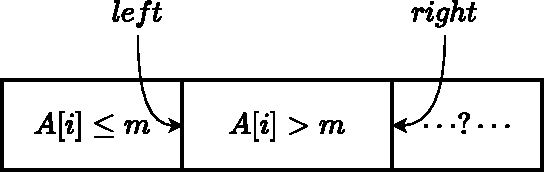
\includegraphics[scale=0.7]{img/partition-by}  % by pdfcrop
  \caption{数组划分。位于$0 \leq i < left$的元素满足$A[i] \leq m$,位于$left \leq i < right$的元素满足$A[i] > m$,剩余的元素尚未处理。}
  \label{fig:divide}
\end{figure}

\section*{正规数}

第二道趣题是如何寻找第1500个正规数。正规数是只含有2、3、5这三种因子的自然数。在数论中叫作5-光滑数。在计算机科学中又叫作哈明数以纪念理查德$\cdot$哈明。2、3、5本身也是正规数。$60 = 2^23^15^1$是第25个正规数。数字$21 = 2^03^17^1$含有因子7,所以不是正规数。定义$1=2^03^05^0$是第0个正规数。前10个正规数如下:

1, 2, 3, 4, 5, 6, 8, 9, 10, 12, ...

\subsection*{穷举法}
我们可以从1开始,逐一检查所有自然数,对每个数把2、3、5这些因子不断去掉,检查最终结果是否为1:

\begin{algorithmic}[1]
\Function{Regular-Number}{$n$}
  \State $x \gets 1$
  \While{$n > 0$}
    \State $x \gets x + 1$
    \If{\Call{Valid?}{$x$}}
      \State $n \gets n - 1$
    \EndIf
  \EndWhile
  \State \Return $x$
\EndFunction
\Statex
\Function{Valid?}{$x$}
  \While{$x \bmod 2 = 0$}
    \State $x \gets x / 2$
  \EndWhile
  \While{$x \bmod 3 = 0$}
    \State $x \gets x / 3$
  \EndWhile
  \While{$x \bmod 5 = 0$}
    \State $x \gets x / 5$
  \EndWhile
  \State \Return $x = 1$ ?
\EndFunction
\end{algorithmic}

随着$n$增大,穷举法用时迅速增加。在同样的计算机上,其C语言实现需要40.39秒才找到第1500个正规数(860934420)。

\subsection*{构造性解法}
取模和除法是耗时的计算\cite{Bentley}。如果不再检查每一个数的因子,而是从2、3、5构造正规数,这样问题就转换为如何从小到大依次产生正规数序列。我们可以使用队列来解决。队列从一侧加入元素,另一侧取出元素。先放入的先被取出。这一特性被称为先进先出FIFO(First In First Out)。先把第0个正规数1加入队列,不断从另一侧取出正规数,分别乘以2、3、5,产生3个正规数并按大小顺序将其加入队列。如果新产生的数已存在于队列中,则丢弃以避免重复。新数可能小于队尾的数,在插入时需要保持它们的大小顺序,如\cref{fig:queues}所示。

\begin{figure}[htbp]
  \centering
  \subcaptionbox{1入队}{\includegraphics[scale=0.5]{img/q1}}
  \hspace{.1\textwidth}
  \subcaptionbox{2、3、5入队}{\includegraphics[scale=0.5]{img/q2}}
  \\
  \subcaptionbox{4、6、10入队}{\includegraphics[scale=0.5]{img/q3}}
  \hspace{.1\textwidth}
  \subcaptionbox{9、15入队,丢弃6}{\includegraphics[scale=0.5]{img/q4}}
  \caption{前4步}
  \label{fig:queues}
\end{figure}

根据这一思路的实现如下:

\begin{algorithmic}[1]
\Function{Regular-Number}{$n$}
  \State $Q \gets [1]$
  \While{$n > 0$}
    \State $x \gets$ \Call{Dequeue}{$Q$}
    \State \Call{Unique-Enqueue}{$Q, 2x$}
    \State \Call{Unique-Enqueue}{$Q, 3x$}
    \State \Call{Unique-Enqueue}{$Q, 5x$}
    \State $n \gets n-1$
  \EndWhile
  \State \Return $x$
\EndFunction
\Statex
\Function{Unique-Enqueue}{$Q, x$}
  \State $i \gets 0, m \gets |Q|$
  \While{$i < m$ 且 $Q[i] < x$}
    \State $i \gets i + 1$
  \EndWhile
  \If{$i \geq m$ 或 $x \neq Q[i]$}
    \State \Call{Insert}{$Q, i, x$}
  \EndIf
\EndFunction
\end{algorithmic}

对于长度为$m$的队列,\textproc{Unique-Enqueue}需要$O(m)$时间按序、无重复地插入新元素。队列的长度随着$n$线性增加(每取出一个后最多插入三个新元素,增加的比率$\leq 2$),总运行时间为$O(1 + 2 + 3 + ... + n) = O(n^2)$。\Cref{fig:big-O-1q}显示了队列的访问次数和$n$之间的关系,形状为二次曲线,反映出$O(n^2)$的复杂度。

\begin{figure}[htbp]
  \centering
  \includegraphics[scale=0.5]{img/big-O-1q}
  \caption{队列访问次数和$n$的关系}
  \label{fig:big-O-1q}
\end{figure}

在同样的计算机上,其C语言实现仅用0.016秒就输出了答案,比穷举法快2500倍。我们也可以用递归实现,令$xs$为包含所有正规数的无穷序列$[x_1, x_2, x_3, ...]$。对每个正规数,将其乘以2得到的仍然是无穷正规数列:$[2x_1, 2x_2, 2x_3, ...]$。同样依次乘以3、5会得到另外两个无穷正规数列。如果将这3个无穷数列合并,去除重复并将1添加到开头,就又得到了$xs$:

\be
  xs = 1 : [2x | x \gets xs] \cup [3x | x \gets xs] \cup [5x | x \gets xs]
\ee

其中$x \cons xs$表示将元素$x$连接到列表$xs$的前面,在Lisp中这个操作称为cons。1是第0个正规数,在最前面。$\cup$合并无穷列表。

\[
(a \cons as) \cup (b \cons bs) = \begin{cases}
  a < b: & a : as \cup (b \cons bs) \\
  a = b: & a : as \cup bs \\
  a > b: & b : (a \cons as) \cup bs \\
\end{cases}
\]

对应的Haskell例子程序:
\begin{Haskell}
xs = 1 : (map (*2) xs) `merge` (map (*3) xs) `merge` (map (*5) xs)

merge (a:as) (b:bs) | a < b = a : merge as (b:bs)
                    | a == b = a : merge as bs
                    | otherwise = b : merge (a:as) bs
\end{Haskell}

通过\texttt{xs !! 1500},可以得到第1500个正规数。在同样的计算机上,这一程序用时0.03秒。

\subsection*{队列}
上面的解法需要排除掉重复元素、扫描队列以保持有序。把所有正规数分成三个类:$Q_2 = \{2^i | i > 0\}$仅包含被2整除的数;$Q_{23} = \{ 2^i3^j | i \geq 0, j > 0 \}$、$Q_{235} = \{ 2^i3^j5^k | i,j \geq 0, k > 0\}$。其中$Q_{23}$要求$j \neq 0$,$Q_{235}$要求$k \neq 0$,保证了三类数间没有重复。每类数都用一个队列来产生。初始化$Q_2=\{ 2 \}$,$Q_{23} = \{ 3 \}$和$Q_{235} = \{ 5 \}$。每次取出三个队列头部的最小元素$x$,然后进行下面的检查:

\begin{itemize}
\item 如果$x$来自$Q_2$,将$2x$加入$Q_2$,$3x$加入$Q_{23}$,$5x$加入$Q_{235}$;
\item 如果$x$来自$Q_{23}$,将$3x$加入$Q_{23}$,$5x$加入$Q_{235}$。我们不应将$2x$加入$Q_2$,因为$Q_2$中不包含被3整除的数。
\item 如果$x$来自$Q_{235}$,将$5x$加入$Q_{235}$。我们不应将$2x$加入$Q_2$,$3x$加入$Q_{23}$,因为它们不包含被5整除的数。
\end{itemize}

不断从三个队列中取出最小的直到第$n$个元素。\cref{fig:q235}给出了前4步。

\begin{figure}[htbp]
  \centering
  \subcaptionbox{4、6、10入队}{\includegraphics[scale=0.5]{img/q235-1}}
  \subcaptionbox{9、15入队}{\includegraphics[scale=0.5]{img/q235-2}} \\
  \subcaptionbox{8、12、20入队}{\includegraphics[scale=0.5]{img/q235-3}} \\
  \subcaptionbox{25入队}{\includegraphics[scale=0.5]{img/q235-4}}
  \caption{使用三个队列$Q_2$、$Q_{23}$、$Q_{235}$构造正规数的前4步。}
  \label{fig:q235}
\end{figure}

\begin{algorithmic}[1]
\Function{Regular-Number}{$n$}
  \State $x \gets 1$
  \State $Q_2 \gets \{ 2 \}$, $Q_{23} \gets \{ 3 \}$, $Q_{235} \gets \{ 5 \}$
  \While{$n > 0$}
    \State $x \gets min$(\Call{Head}{$Q_2$}, \Call{Head}{$Q_{23}$}, \Call{Head}{$Q_{235}$})
    \If{$x =$ \Call{Head}{$Q_2$}}
      \State \Call{Dequeue}{$Q_2$}
      \State \Call{Enqueue}{$Q_2, 2x$}
      \State \Call{Enqueue}{$Q_{23}, 3x$}
      \State \Call{Enqueue}{$Q_{235}, 5x$}
    \ElsIf{$x=$ \Call{Head}{$Q_{23}$}}
      \State \Call{Dequeue}{$Q_{23}$}
      \State \Call{Enqueue}{$Q_{23}, 3x$}
      \State \Call{Enqueue}{$Q_{235}, 5x$}
    \Else
      \State \Call{Dequeue}{$Q_{235}$}
      \State \Call{Enqueue}{$Q_{235}, 5x$}
    \EndIf
    \State $n \gets n - 1$
  \EndWhile
  \State \Return $x$
\EndFunction
\end{algorithmic}

算法循环$n$次。每次从三个队列中取出最小元素,这一步需要常数时间。接着根据取出元素所在的队列,产生一到三个新数加入队列,这一步也是常数时间。整个算法复杂度为$O(n)$。

\section*{小结}
尽管两道趣题都能用穷举法解决,但随着规模增加,我们不得不寻求更好的解法。本书介绍常见的基本算法和数据结构,同时给出函数式和命令式的对比实现。主要参考了冈崎的著作\cite{okasaki-book}和经典的算法教材\cite{CLRS}。本书尽量避免依赖于特定的编程语言。一方面读者会有自己的偏好,另一方面编程语言也在不断变化。为此我们主要使用伪代码和数学记法对算法进行定义,并附以一些例子代码。函数式的示例类似Haskell,命令式的示例是几种语言的混合体。

本书中文版《算法新解》从2009年开始写作,2017年出版。2020年底开始重写,2022年2月完成了第二版。电子版可以在github上获得,如果希望获得纸质版,请在github上联系我。

\begin{Exercise}\label{ex:preface}
\Question{最小可用数趣题中,所有数都是非负整数。我们可以利用正负号来标记一个数字是否存在。首先扫描一遍列表,令列表长度为$n$,对于任何绝对值小于$n$的数$|x| < n$,将位置$|x|$上的数字置为负数。之后再次扫描一遍列表,找到第一个正数所在的位置就是答案。编程实现这一算法。}

\Question{$n$个数字1, 2, ..., $n$,经过某一处理后,它们的顺序被打乱了,并且某一个数$x$被改成了$y$。假设$1 \leq y \leq n$,设计一个方法能够在线性时间、常数空间内找出$x$和$y$。}

\Question{下面是一段求正规数的代码。它是一种队列解法么?
\begin{lstlisting}[language = Bourbaki]
Int regularNum(Int m) {
    [Int] nums(m + 1)
    Int n = 0, i = 0, j = 0, k = 0
    nums[0] = 1
    Int x2 = 2 * nums[i]
    Int x3 = 3 * nums[j]
    Int x5 = 5 * nums[k]
    while n < m {
        n = n + 1
        nums[n] = min(x2, x3, x5)
        if x2 == nums[n] {
            i = i + 1
            x2 = 2 * nums[i]
        }
        if x3 == nums[n] {
            j = j + 1
            x3 = 3 * nums[j]
        }
        if x5 == nums[n] {
            k = k + 1
            x5 = 5 * nums[k]
        }
    }
    return nums[m]
}
\end{lstlisting}
}
\end{Exercise}

\begin{Answer}[ref={ex:preface}]
\Question{最小可用数趣题中,所有数都是非负整数。我们可以利用正负号来标记一个数字是否存在。首先扫描一遍列表,令列表长度为$n$,对于任何绝对值小于$n$的数$|x| < n$,将位置$|x|$上的数字置为负数。之后再次扫描一遍列表,找到第一个正数所在的位置就是答案。编程实现这一算法。

\begin{Bourbaki}
Int minFree([Int] nums) {
    var n = length(nums)
    for Int i = 0 to n {
        var k = abs(nums[i])
        if k <= n then nums[k - 1] = -abs(nums[k - 1])
    }
    for Int i = 0 to n {
        if nums[i] > 0 then return i + 1
    }
    return n + 1
}
\end{Bourbaki}
}

\Question{$n$个数字1, 2, ..., $n$,经过某一处理后,它们的顺序被打乱了,并且某一个数$x$被改成了$y$。假设$1 \leq y \leq n$,设计一个方法能够在线性时间、常数空间内找出$x$和$y$。

例如$X$ = [3, 1, 3, 5, 4]中,丢失的是$x = 2$,重复的是$y = 3$。我们给出4种解法:(1)分治、(2)鸽笼排序、(3)符号编码、(4)解方程。

\textbf{分治}方法。使用中点$m = \lfloor \dfrac{1 + n}{2} \rfloor$划分序列为两部分,左侧:$as = [a \leq m, a \gets X]$、右侧:$bs = [b > m, b \gets X]$。如果左侧长度$|as| < m$,可知丢失的数字在左侧,记$s = 1 + 2 + ... + m = \dfrac{m (m + 1)}{2}$,则$x = s - sum(as)$。同时可计算出重复的数字在右侧,记$s' = (m + 1) + (m + 2) + ... + n = \dfrac{(n + m + 1)(n - m)}{2}$,则$y = sum(bs) - s'$;若左侧的长度$|as| > m$,可知重复的数字在左侧。使用同样的方法,可以算出丢失的数字$x = s' - sum(bs)$,重复的数字$y = sum(as) - s$;否则,如果左侧的长度$|as| = m$,说明有$m$个不大于$m$的数字,但我们不知道它们是否是1, 2, ..., $m$的某个排列。为此,我们可以计算并比较$sum(as)$和$s$。如果相等,说明左侧没有问题,可以丢弃左侧的所有数字,然后递归地在右侧寻找$x$和$y$;否则,我们丢弃右侧,在左侧递归寻找答案。在递归查找时,需要用序列的下限$l$替换上述步骤中的1。由于每次去掉一半的列表,根据主定理,总时间复杂度为$O(n)$。或通过等比数列推导复杂度:$O(n + n/2 + n/4 + ...) = O(2n) = O(n)$。

\begin{Haskell}
missDup xs = solve xs 1 (length xs) where
  solve xs@(_:_:_) l u | k < m - l + 1 = (sl - sl', sr' - sr)
                       | k > m - l + 1 = (sr - sr', sl' - sl)
                       | sl == sl' = solve bs (m + 1) u
                       | otherwise = solve as l m
      where
          m = (l + u) `div` 2
          (as, bs) = partition (<=m) xs
          k = length as
          sl = (l + m) * (m - l + 1) `div` 2
          sr = (m + 1 + u) * (u - m) `div` 2
          (sl', sr') = (sum as, sum bs)
\end{Haskell}

\textbf{鸽笼排序}。由于所有的数字都在1到$n$之间,我们可以使用鸽笼排序来重新排列数字。我们自左向右扫描,对于每个位置$i$上的数字$x$,如果$x \neq i$,我们就将它和位置$x$上的数字$y$交换。如果$x = y$,我们就找到了重复的数字,同时,我们得知丢失的数字就是$i$,重复这一交换过程,直到$x$等于$i$或者找到重复的数字。由于每个数字仅被交换一次以到达正确的位置,因此总时间复杂度为$O(n)$。

\begin{Bourbaki}
(Int, Int) missDup([Int] xs) {
    (Int miss, Int dup) = (-1, -1)
    for Int i = 0 to length(xs) - 1 {
        while xs[i] != i {
            Int j = xs[i]
            if xs[j] == xs[i] {
                dup = xs[j]
                miss = i
                break
            } else {
                j = xs[i]
                (xs[i], xs[j]) = (xs[j], xs[i])
            }
        }
    }
    return (miss, dup)
\end{Bourbaki}

\textbf{符号编码}。假设存在一个长度为$n$的标记数组,对于序列中的每个数字$x$,我们都将标记数组中的第$x$个位置做上标记。当我们遇到重复元素时,我们会发现这个位置上的标记已经做过了。记重复的数字为$d$,我们知道$s = 1 + 2 + ... + n = \dfrac{n (n + 1)}{2}$,以及序列中所有的数字和$s'$。我们可以计算出丢失的数字$m = d + s - s'$。 但是这一方法需要额外长度为$n$的空间用作标记数组。由于数字的存在与否是一种二值化的信息(有、无),我们可以将其编码为数字的正负号,从而复用待查找的数字序列。对于序列中的每个数字$x$,我们将序列中第$|x|$位置上的元素标记为负数,其中$|x|$表示$x$的绝对值。如果发现某一位置已经为负了,我们就找到了重复的元素,接下来我们就可以计算出丢失的数字。

\begin{Bourbaki}
(Int, Int) missDup([Int] xs) {
    (Int miss, Int dup) = (-1, -1)
    Int n = length(xs)
    Int s = sum(xs)
    for i = 0 to n - 1 {
        Int j = abs(xs[i]) - 1
        if xs[j] < 0 {
            dup = j
            miss = dup + n * (n + 1) / 2 - s
            break
        }
        xs[j] = - abs(xs[j])
    }
    return (miss, dup)
\end{Bourbaki}

\textbf{解方程}。考虑一个简化的问题:给定一个从1到$n$的列表,去掉一个元素,然后打乱序列的顺序,怎样能够快速找出去掉的元素呢?我们可以将列表中所有的元素相加,然后从$\dfrac{n (n + 1)}{2}$减去这一结果就得出了答案。这一思路可以表示为如下方程:

\[
m = s - s'
\]

其中$m$表示丢失的数字,$s$是从1到$n$的累加和,$s'$是列表中所有元素的和。但是同时存在丢失的元素和重复的元素,无法仅用一个方程求出两个未知数。

\be
\sum (x[i] - i) = d - m
\label{eq:miss-dup-1}
\ee

其中左侧是列表中第$i$个元素减去$i$后的累加和。能否找出第二个独立的方程呢?思路是使用平方。如果我们将第$i$个元素的平方减去$i$的平方,然后将结果累加起来。就可以得到下面的结果:

\be
\sum (x[i]^2 - i^2) = d^2 - m^2 = (d + m)(d - m)
\label{eq:miss-dup-2}
\ee

由于$d - m$不等于0,我们可以用式(\cref{eq:miss-dup-1})除以式(\cref{eq:miss-dup-2})两侧,得到另一个方程:

\be
\sum (x[i]^2 - i^2) / \sum (x[i] - i) = d + m
\label{eq:miss-dup-3}
\ee

比较方程(\cref{eq:miss-dup-1})和方程(\cref{eq:miss-dup-3}),两个方程、两个未知数,这样就可以得到结果:

\[
\begin{cases}
m = \dfrac{1}{2} (\dfrac{\sum (x[i]^2 - i^2)}{\sum (x[i] - i)} - \sum (x[i] - i)) \\
d = \dfrac{1}{2} (\dfrac{\sum (x[i]^2 - i^2)}{\sum (x[i] - i)} + \sum (x[i] - i)) \\
\end{cases}
\]

\begin{Haskell}
missDup xs = ((b `div` a - a) `div` 2, (b `div` a + a) `div` 2) where
  ys = zip xs [1..]
  a = sum [x - y | (x, y) <- ys]
  b = sum [x^2 - y^2 | (x, y) <- ys]
\end{Haskell}
}

\Question{是的,它是一种等价的队列解法。}
\end{Answer}

\ifx\wholebook\relax \else
\section*{参考答案}
\shipoutAnswer

\begin{thebibliography}{99}

\bibitem{fp-pearls}
Richard Bird. ``Pearls of functional algorithm design''. Cambridge University Press; 1 edition (November 1, 2010). ISBN-10: 0521513383. pp1 - pp6.

\bibitem{Bentley}
Jon Bentley. ``Programming Pearls(2nd Edition)''. Addison-Wesley Professional; 2 edition (October 7, 1999). ISBN-13: 978-0201657883 (中文版:《编程珠玑》)

\bibitem{okasaki-book}
Chris Okasaki. ``Purely Functional Data Structures''. Cambridge university press, (July 1, 1999), ISBN-13: 978-0521663502

\bibitem{CLRS}
Thomas H. Cormen, Charles E. Leiserson, Ronald L. Rivest and Clifford Stein. ``Introduction to Algorithms, Second Edition''. The MIT Press, 2001. ISBN: 0262032937. (中文版:《算法导论》)

\end{thebibliography}

\expandafter\enddocument
\fi
